\section{Performance comparison} 
\label{sec:performance_comparison}

In this section we present some results obtained using the described robust planning frameworks. All planned trajectories refer to the sector of the Catalunya circuit shown in Figure~\ref{fig:track}. 
The entire circuit is parametrized by the curvilinear abscissa $\alpha \in [0,1]$, and the selected sector corresponds to the interval $\left[0.70, 0.77\right]$. Checkpoints are indicated by labels and are uniformly spaced by $\De\al=0.01$. This sector includes two distinct corners: a low-speed turn from $\al = 0.72$ to $\al = 0.73$, and a high-speed turn from $\al = 0.75$ to $\al = 0.76$, allowing for the evaluation of vehicle behavior across different dynamic scenarios.

We begin by presenting a selection of results obtained with the open-loop planning approach, which allows for a clearer illustration of the method and its underlying mechanisms. This approach is used as a reference to analyze the influence of key design parameters and of the different types of constraints on the resulting trajectories. A comparison is then carried out between the open-loop and closed-loop strategies. Finally, the planned trajectories are compared against those followed in simulations with noise realizations, providing empirical validation of the proposed framework.

% Contour plot dei LAP time in funzione dei due gamma, lo mettiamo o no? Eventialmente nel comparison open/closed

\begin{figure}
	\centering
	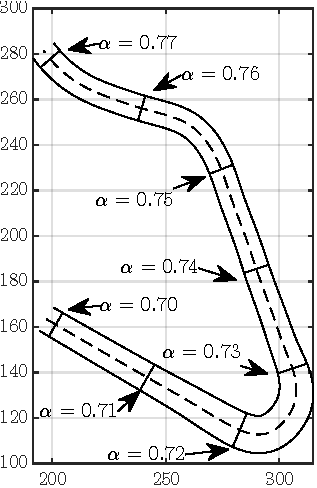
\includegraphics{Fig/track.pdf}
	\caption{Sector of the Catalunya circuit considered in the analysis, corresponding to the curvilinear abscissa interval $\left[0.70, 0.77\right]$. Checkpoints are indicated by labels and are uniformly spaced by $\De\al=0.01$. This sector includes two distinct corners: a low-speed turn from $\al = 0.72$ to $\al = 0.73$, and a high-speed turn from $\al = 0.75$ to $\al = 0.76$, allowing for the evaluation of vehicle behavior across different dynamic scenarios.}
	\label{fig:track}
\end{figure}

\subsection{Open-loop parameters sensitivity}
\label{sec:ol_param_sensitivity}
To gain deeper insight into how key parameters affect the planning outcome, we focus here on the open-loop formulation.
%In this section, we explore the open-loop approach to gain deeper insight into the influence of key parameters on the results.
At this stage, only the track limit constraint is robustified. 
%For this analysis, we consider optimizations in which only the track limit constraint is robustified. 
This choice is motivated by the fact that its effects are more visually evident than those of the friction limit constraint, thereby facilitating a more immediate understanding of their impact. 

The first parameter considered is the confidence level of constraint satisfaction. 
We recall that the factor $\ga^\textrm{TLC}$ acts as a tuning knob, multiplying the standard deviation of the constraint, $\sigma^\textrm{TLC}$, to determine the total back-off term $\be^\textrm{TLC}$. 
This parameter directly influences the probability of satisfying the track limit constraint: higher values of $\ga^\textrm{TLC}$ correspond to more conservative (i.e., robust) behavior. 
Specifically, $\ga^\textrm{TLC} = 0$ yields a satisfaction probability of 50\% and leads to the nominal solution with no back-off, while $\ga^\textrm{TLC} = 3$ corresponds to a confidence level of 99\%. 
For the purposes of this analysis, we examine the effect of varying $\ga^\textrm{TLC}$ across this range. 

%Setting $\ga^\textrm{TLC} = 0$ leads to the nominal solution. In this case, the back-off term $\be^\textrm{TLC}$ becomes zero, meaning that the constraint is not robustified and thus coincides with the original, non-robust formulation. 

Observing the left panel of Figure~\ref{fig:ol_sensitivities}, it is evident that the trajectories corresponding to configurations with lower values of $\ga^\textrm{TLC}$ tend to travel closer to the track boundaries. In contrast, the trajectory associated with $\ga^\textrm{TLC} = 3$---represented by the light green line---remains significantly farther from the edges.
This behavior is consistent with the increased conservativeness introduced by higher values of $\ga^\textrm{TLC}$, which amplify the back-off term $\be^\textrm{TLC}$ and thereby enforce a larger safety margin from the track limits.
Chasing a trajectory associated with a larger safety margin leads to higher sector times; spanning $\ga^\textrm{TLC}$ in the range $\left[0,3\right]$ results in sector times that vary from 12.135\,s to 13.162\,s.

\begin{figure}
	\centering
	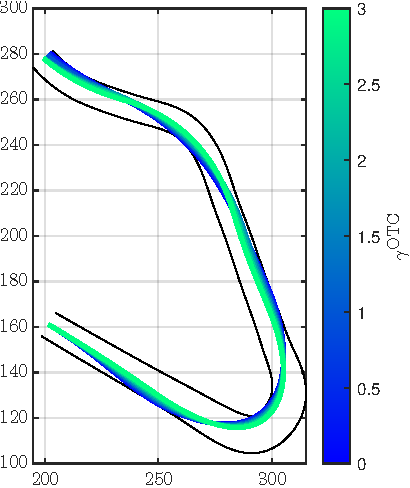
\includegraphics{Fig/gamma_sensitivity.pdf}
	\hfill
	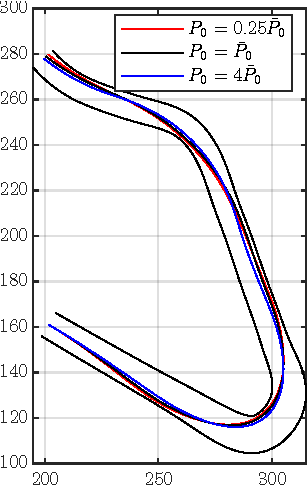
\includegraphics{Fig/Pzero_sensitivity.pdf}
	\caption{Effect of $\ga^\textrm{TLC}$ (left panel) and $P_0$ (right panel) on optimal trajectory. The parameter $\ga^\textrm{TLC}$ spans in the range $\left[0,3\right]$ corresponding to a probability to meet the track limit constraint ranging from 50\% to 99\%. In the right panel, in addition to the baseline value $\bar{\bP}_0$ (black line), two alternative values are considered: $\bP_0 = 4\bar{\bP}_0$ (blue line) and $\bP_0 = \frac{1}{4}\bar{\bP}_0$ (red line). These correspond, respectively, to doubling and halving the initial uncertainty associated with the state vector.}
	\label{fig:ol_sensitivities}
\end{figure}

The second parameter examined is the initial value of the covariance matrix, $\bP_0$. 
We recall that at each grid point a new prediction horizon is initialized, and the corresponding matrix $\bP$ at its starting point, i.e., $\bP^0_k$, is set to $\bP_0$. 
The diagonal elements of $\bP$ are the variances $\text{var}(x_i)$ of each state variables, while the off-diagonal elements encode their covariances $\text{cov}(x_i,x_j)$. Larger diagonal values indicate higher uncertainty in the corresponding states, and nonzero off-diagonal terms imply mutual dependence between them. For simplicity, a diagonal $\bP_0$ is used in this study, that is, for each prediction horizon we assign an initial standard deviation $\sigma_i = \sqrt{\text{var}(x_i)}$ to each state and assume all initial covariances to be zero. 

To provide a concrete interpretation, consider the first state variable $x_1$ with mean $\mu_1$ and standard deviation $\sigma_1$.
Under the Gaussian assumption, the true value of $x_1$ lies within the interval $\left[\mu_1 - \sigma_1,\ \mu_1 + \sigma_1\right]$ with approximately 68\% probability, and within the interval $\left[\mu_1 - 3\sigma_1,\ \mu_1 + 3\sigma_1\right]$ with approximately 99\% probability.

We assign a baseline initial covariance matrix $\bP_0 = \bar{\bP}_0$ by selecting standard deviations $\bar{\sigma}_i$ for each state variable. These standard deviations have been chosen based on the typical range of variation of each state.
Assuming the state vector is ordered as described in Section~\ref{sec:vehicle_model}, the values used are $\bar{\boldsymbol{\sigma}}~=~\left[0.1\,\textrm{m/s}, 0.01\,\textrm{m/s}, 0.01\,\textrm{rad/s}, 1\,\textrm{m}, 1\,\textrm{m}, 0.0175\,\textrm{rad}\right]^T$.
In addition to the baseline value $\bar{\bP}_0$, two alternative values are considered: $\bP_0 = 4\bar{\bP}_0$ and $\bP_0 = \frac{1}{4}\bar{\bP}_0$. These correspond, respectively, to doubling and halving the initial standard deviations $\sigma_i$ associated with the state vector. 

A comparison between the trajectories obtained using different values of $\bP_0$ is shown in the right panel of Figure~\ref{fig:ol_sensitivities}.
The black line corresponds to the baseline case with $\bP_0 = \bar{\bP}_0$, while the red and the blue lines represent the cases with $\bP_0 = \frac{1}{4}\bar{\bP}_0$ and $\bP_0 = 4\bar{\bP}_0$, respectively. As reasonably expected, using a larger initial covariance matrix results in a greater covariance matrix after $H$ steps, which in turn leads to a higher back-off term. This is reflected in the blue line, which travels closer to the centerline with respect to the other two lines.

\subsection{Robustified constraints comparison}
%It is of interest to analyze how a robustified constraint---or a combination of the two described in Sections~\ref{sec:FLC} and~\ref{sec:TLC}---influences the driving style. 
We now investigate how the inclusion of different kinds of robustified constraints---individually or in combination, as described in Sections~\ref{sec:FLC} and~\ref{sec:TLC}---influences the driving style. 
We compare the nominal feed-forward optimal trajectory, obtained without robustified constraints, with those resulting from a robustified track limit constraint (denoted as TLC), a robustified friction limit constraint (denoted as FLC), and a scenario where both constraints are robustified (denoted as TLC+FLC). All the optimization are obtained with the open-loop method described in Section~\ref{sec:open_loop_planning}, setting $H=4$, and $\ga^\textrm{TLC}=\ga^\textrm{FLC}=1.28$, corresponding to a 90\% probability of satisfying both constraints. 

\begin{figure}
	\centering
	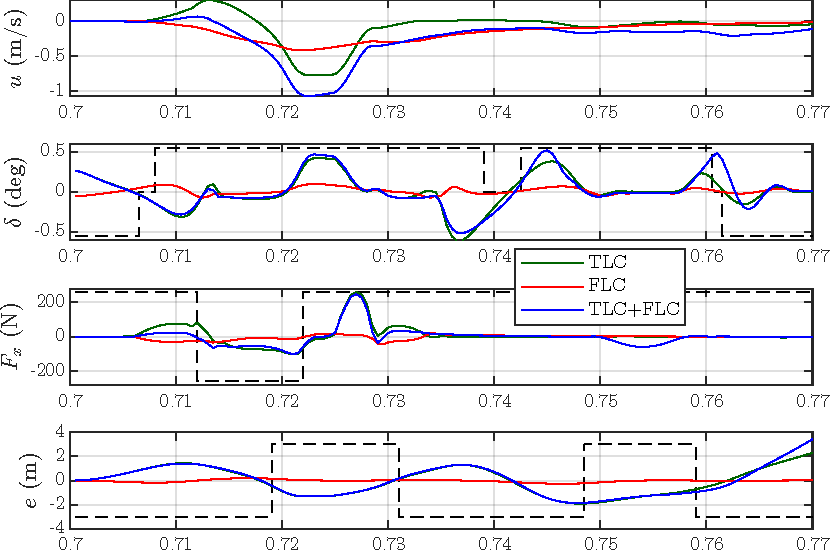
\includegraphics{Fig/ol_telemetries.pdf}
	\caption{Evolution of the longitudinal speed $\De u$, wheel steering angle $\De \de$, longitudinal force $\De F_x$, and lateral deviation $\De e$ are reported for three robustification scenarios: TLC (Track Limit Constraints), FLC (Friction Limit Constraint), and TLC+FLC (both constraints enforced concurrently). Each profile is shown relative to the baseline (nominal) trajectory to highlight the effect of each constraint-handling strategy. The dashed lines in the last three panels indicate the sign of the reference signal, allowing one to determine whether a positive variation with respect to the baseline corresponds to an increase or a decrease in the absolute value. This distinction is particularly important for quantities that depend on the direction of the turn, such as the wheel steering angle $\de$ and the lateral deviation $e$, while in the case of $F_x$, it indicates whether the vehicle is accelerating or braking.}
	\label{fig:ol_telemetries}
\end{figure}

%---Delta key signals

The comparison between the nominal case and the three robustified cases is illustrated in Figure~\ref{fig:ol_telemetries}, in terms of the deviation of selected signals from to their nominal counterparts.
The panels display variations on the longitudinal speed $\De u$ (first panel), wheel steering angle $\De \de$ (second panel), total longitudinal force $\De F_x$ (third panel), and lateral deviation of the center of mass (CoM) from the track centerline $\De e$ (fourth panel). 
Except for the $\De u$ panel, each plot includes dashed black lines that indicate the sign of the nominal signal. 
These indicators are shown at three distinct vertical levels---upper, central, and lower---corresponding respectively to positive, near-zero, and negative values of the nominal signal.

%--------1 Considerazioni generali sul settore

From the first panel, it can be observed that all robustified configurations, on average, show a lower longitudinal speed compared to the nominal trajectory, resulting in an increased sector time. Specifically, the configuration with the robustified TLC increases the sector time by 1.66\%, while that with the robustified FLC leads to a 0.79\% increase. When both TLC and FLC are robustified, the sector time increases by 2.57\%.
The two configurations incorporating the robustified TLC (blue and green lines) exhibit, as expected, a significantly altered CoM trajectory.
Ideed, the second and fourth panels clearly show that the TLC and TLC+FLC configurations tend to follow a path closer to the centerline. In particular, for most of the sector, the variation in lateral displacement $\De e$ and the lateral displacement $e$ itself exhibit opposite signs, indicating a corrective behavior of the steering angle $\de$ that pulls the vehicle toward the centerline.

%--------2 Sharp turn

This shift in trajectory and longitudinal speed becomes especially evident when approaching the sharp turn at $\al \in [0.707, 0.712]$. A noticeable increase in longitudinal speed is observed around $\alpha = 0.71$ for the TLC configuration  in the $\De u$ panel. This peak is followed by a sharp drop in speed, indicating intense braking.
The TLC+FLC configuration exhibits a qualitatively similar trend in $\Delta u$, although the peak is significantly lower and the subsequent speed reduction is clearly stronger. This behavior is consistent with the variation of the total longitudinal force $\Delta F_x$ shown in the third panel.
In particular, the TLC and TLC+FLC configurations exhibit a higher longitudinal force while approaching the sharp turn, in the curvilinear abscissa interval $\al\in\left[0.707, 0.712\right]$, resulting in a higher longitudinal speed.
Subsequently, these two configurations apply a lower longitudinal force during braking compared to the nominal case, indicating more intense braking. This behavior explains the sharp reduction in longitudinal speed observed thereafter.

%--------3 High speed turn

Later in the sector, a further deviation in driving style appears during the high-speed turn, specifically around $\alpha \in [0.75, 0.76]$.
As shown in the $\Delta F_x$ panel, the combined configuration TLC+FLC needs to reduce the longitudinal force within this section to meet both the constraints. 
This adaptation is necessary because the TLC forces the vehicle to follow a wider trajectory, which entails greater lateral acceleration and, consequently, higher lateral force demand. To satisfy the FLC under the resulting increase in tire utilization, the available accelerating force must be reduced.
Based on the nominal force sign indicator, this reduction is achieved by partially lifting the throttle.

%---Axle saturation
After analyzing the variations of these four key signals with respect to the nominal solution, we now turn our attention to the evaluation of axle saturation, which provides insight into how close each configuration operates to the tire grip limits. 
In accordance with the FLC formulation introduced in~\ref{eq:adherence_constraint}, we define the \emph{axle saturation ratio} $S_j$ as
\begin{equation}
	S_j = \frac{ \left( \frac{X_j(\bx,\bu)}{\mu_{x,j}} \right)^2+ \left( \frac{Y_j(\bx,\bu)}{\mu_{y,j}}\right)^2}{Z_j^2(\bx,\bu)}.
\end{equation}
This quantity indicates how close each configuration operates to the friction limit; $S_j = 1$ when the point $\left(X_j, Y_j\right)$ lies exactly on the friction ellipse, i.e., under full saturation.
Figure~\ref{fig:ol_saturation} shows the values of $S_j$ for the front axle ($j=1$, first panel) and the rear axle ($j=2$, rear panel) for the previously introduced configurations: the nominal case (black dashed line) and the three robustified cases (color-coded as before).

\begin{figure}
	\centering
	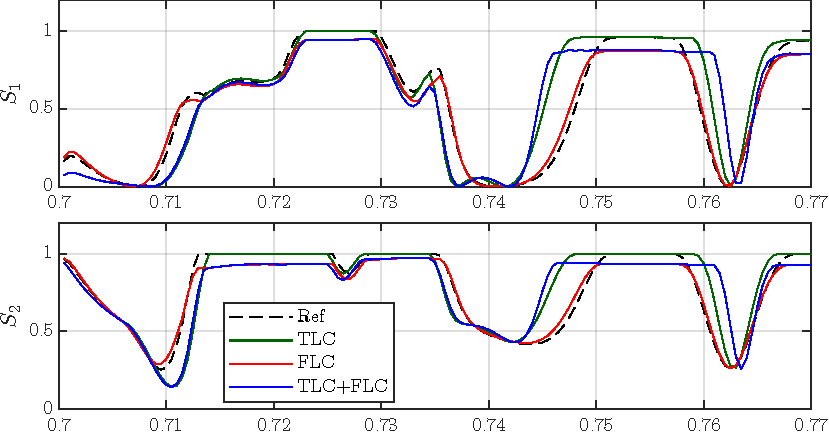
\includegraphics{Fig/ol_saturation.pdf}
	\caption{Tire usage for front axle (first panel) and rear axle (second panel) over curvilinear abscissa $\al$. The plotted lines represent the quantity $\left[ \left( \frac{X_j(\bx,\bu)}{\mu_{x,j}} \right)^2+ \left( \frac{Y_j(\bx,\bu)}{\mu_{y,j}}\right)^2\right]\frac{1}{Z_j^2(\bx,\bu)}$, where $j=1$ denotes the front axle and $j=2$ the rear axle. The dashed black line corresponds to the reference (nominal) configuration, while the green, red, and blue lines represent the robust configurations TLC, FLC, and TLC+FLC, respectively.}
	\label{fig:ol_saturation}
\end{figure}

First, we observe that the FLC and TLC+FLC configurations (red and blue lines) never reach full saturation, i.e., $S_j=1$, due to the presence of the back-off term, which enforces a safety margin from the friction limit. 
Second, we point out how the different trajectories followed by the TLC and TLC+FLC configurations (green and blue lines), compared to the nominal and FLC cases, entail distinct ground force demands, which are clearly visible here in terms of the $S_j$ ratio.
This behavior emerges around the sharp turn and becomes even more evident in the high-speed turn. 
Specifically, in the interval $\alpha \in [0.745, 0.762]$, the TLC and TLC+FLC configurations begin to experience high axle loads approximately 12\,m before the nominal trajectory and sustain them for an additional 4.6\,m (TLC, green line) and 9.2\,m (TLC+FLC, blue line) beyond the nominal reference. 


%As already observed, the configurations with the robustified track limit constraint (green and blue lines) follow significantly different paths compared to the nominal solution. This deviation results in distinct ground force demands, clearly visible in the saturation index.
%From this plot, it can be observed that the configurations with the robustified track limit constraint (green and blue lines) follow significantly different trajectories compared to the nominal solution, resulting in distinct ground force demands. This behavior is noticeable in turn 1 and even more clearly in turn 2. Specifically, these two configurations begin to experience high axle loads approximately 12\,m before the nominal trajectory and sustain them for an additional 4.6\,m (TLC, green line) and 9.2\,m (TLC+FLC, blue line) beyond the nominal reference. 

\subsection{Comparison between open-loop and closed-loop approaches}

\subsection{Simulations with noise realization}
This analysis aims to provide empirical validation of the robust trajectories obtained using the methods proposed in this work. For conciseness, the comparison is limited to a nominal trajectory and a trajectory computed using the closed-loop method with only the track limit constraint robustified.
An LQR controller, designed according to the procedure outlined in Section~\ref{sec:LQR}, is implemented to stabilize the nominal trajectory. In contrast, the robust trajectory is tracked using the controller directly obtained from the optimization process. 

\begin{figure}
	\centering
	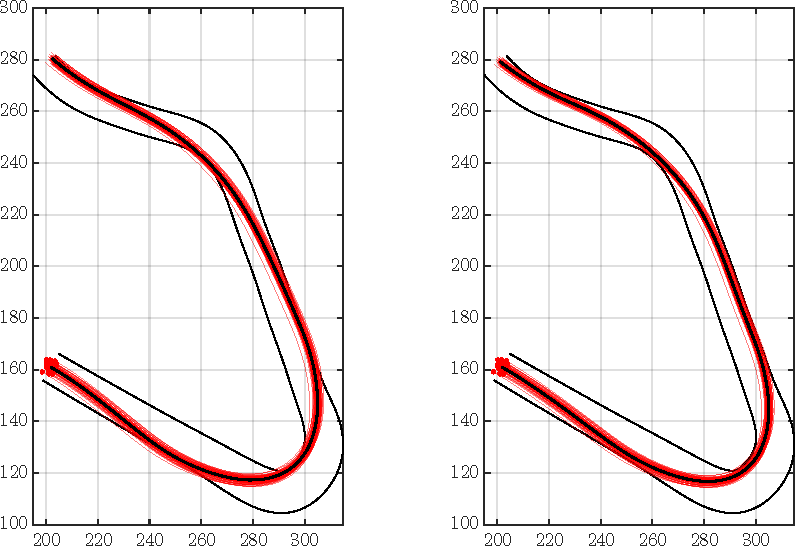
\includegraphics{Fig/olcl_traj_strings.pdf}
	\caption{Simulations with random initial conditions and Gaussian noise realizations. In the left panel, the reference trajectory is the non-robust one, tracked using an LQR controller designed around it. In the right panel, the reference is a robust trajectory obtained using the closed-loop optimization method, and it is tracked using the corresponding optimized controller produced by the same method.}
	\label{fig:traj_strings}
\end{figure}